\documentclass[12pt, titlepage]{article}
\usepackage{xcolor} % for different colour comments

%% Comments
\newif\ifcomments\commentstrue

\ifcomments
\newcommand{\authornote}[3]{\textcolor{#1}{[#3 ---#2]}}
\newcommand{\todo}[1]{\textcolor{red}{[TODO: #1]}}
\else
\newcommand{\authornote}[3]{}
\newcommand{\todo}[1]{}
\fi

\newcommand{\wss}[1]{\authornote{magenta}{SS}{#1}}
\newcommand{\ds}[1]{\authornote{blue}{DS}{#1}}

%% Graphics
\usepackage{float}
\usepackage{caption}
\usepackage{graphicx}
\usepackage{courier}
\graphicspath{ {images/} }

\begin{document}

\title{Smart Waiter User Guide} 
\author{Meraj Patel \#1137491 \\ Pavneet Jauhal \#1149311\\ Shan Perera \#1150394}
\date{\today}
\maketitle

\tableofcontents 

\listoftables

\begin{table}[H]
\section*{Revision History}
\begin{tabular}{|c|c|}
\hline
\textbf{Date}  & \textbf{Comments} \\ \hline
February 26, 2016 &  First Draft. \\ 
\hline
February 27, 2016 & Create Account section complete. \\
\hline
February 28, 2016 & Account Setup complete \\
\hline
February 28, 2016 & Placing an Order complete \\
\hline
February 29, 2016 & All sections complete \\
\hline
\end{tabular}
\caption{Revision History Table}
\end{table}



\section{Introduction}

\subsection{What is Smart-Waiter?}
Smart-Waiter is an application that aims to provide a solution to allow users to order and pay through a mobile application at restaurants. More specifically, it allows users to walk into a restaurant, scan a code to view the menu, and proceed to order and pay for their meal.
\subsection{Objectives of User Manual}
This document describes how to use Smart-Waiter mobile application. For the scope of this project, this guide is written for restaurant patrons. This manual will describe instructions necessary for a user to walk into a restaurant and place an order using Smart-Waiter application. 

\subsection{System Requirements}
To use Smart-Waiter, your phone must be running Android's Ice Cream Sandwich (4.0.1) operating system or higher. Your device must also have at least 512MB of RAM. 
\ds{That seems like a lot.}
The minimum and recommended requirements for running Smart-Waiter are given below.
Minimum Requirements:
\begin{enumerate}
	\item Android OS Version: Ice Cream Sandwich (4.0.1)
	\item Resolution: 480 x 854 pixels (~195 PPI pixel density)
	\item Processor: 1.0 GHz
	\item Storage: 100MB
	\item RAM: 512MB
	\item Camera: 2.0 MP Front Facing Camera
	\item WLAN: WiFi 802.11 b/g/n OR HSPA compatible data service
\end{enumerate}

Recommended Requirements:
\begin{enumerate}
\item Android OS Version: Marshmallow (6.0)
	\item Resolution: 1440 x 2560 pixels (~575 PPI pixel density)
	\item Processor: Exynos 7420 Octacore (1.5 GHz Quad Core \& 2.1 GHz Quad Core)
	\item Storage: 100MB
	\item RAM: 3GB \ds{Have you actually done tests showing you need this much RAM?}
	\item Camera: 16.0 MP Front Facing Camera
	\item WLAN: WiFi 802.11 b/g/n OR LTE compatible data service	
\end{enumerate}

\subsection{Installation Instructions}
Instructions for installing Smart-Waiter with 3 different methods are presented below. Currently, the only way to install Smart-Waiter is through Android Studio. Once the final revision is complete, installation using the application APK or through the Play Store will be available.

\textbf{\newline Installation through the Play Store:}
	\begin{enumerate}
		\item Open the Play Store application on your device.
		\item Press the Search Button
		\item Enter \emph{Smart Waiter} into the search field.
		\item Select \emph{Smart Waiter} from the search results.
		\item Press the \texttt{Install} button.		
	\end{enumerate}

\textbf{\newline Installation with APK:}
	\ds{You should mention they will need a file explorer on their device (does not come standard)}
	\begin{enumerate}
		\item Download the APK file from the Smart-Waiter Git Repository
		\item Open your device's \emph{File Explorer} application
		\item Navigate to the folder where the APK file was saved
		\item Open the APK file using your device's \emph{File Explorer}
		\item Press the \texttt{Install} button
	\end{enumerate}

\textbf{\newline Installation with Android Studio:}
	\begin{enumerate}
		\item Checkout the Smart-Waiter Git Repository to a directory of 				your choice
		\item Open \emph{Android Studio}
		\item Select the \texttt{File} tab from the Menu
		\item Select \texttt{New Project >> Import Project...}
		\item Navigate to the folder where Smart-Waiter is saved
		\item Select the \texttt{build.gradle} file in the \emph{root} 					directory
		\item Wait for the project to build
		\item Plug your Android device in to your computer 
		\item Press the \texttt{Run 'app'} button or a \texttt{Shift+F10}
		\item Select your Android device from the \emph{Choose a running device} section
		\begin{center}
			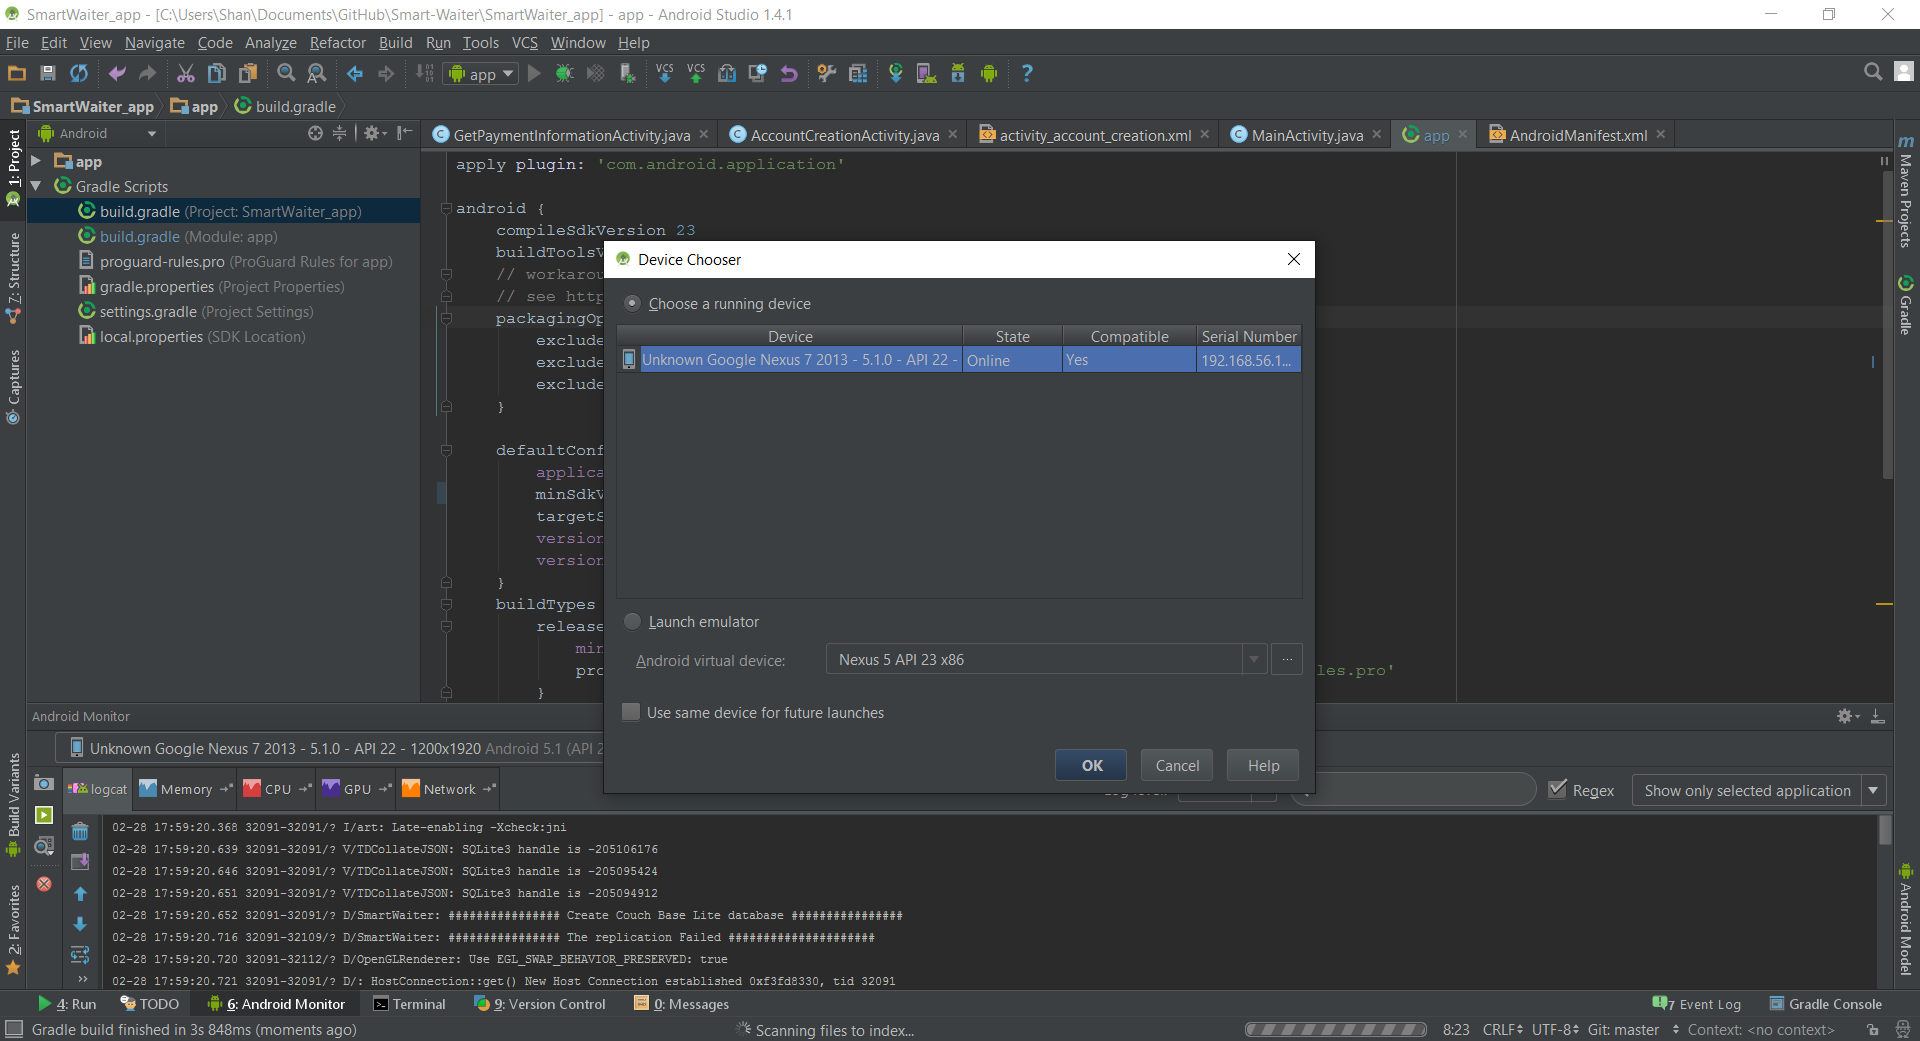
\includegraphics[width=1.0\textwidth]{android-studio.png}
			\linebreak Figure 1 \ds{Use captions and label figures descriptively.}
		\end{center}
		\item Press the \texttt{OK} button		
	\end{enumerate}
You have successfully installed Smart-Waiter on your Android device.

\section{Account Setup}
\subsection{Creating an Account}
If this is the first time that Smart-Waiter is launched, you will be asked to create an account. You will be brought to the Account Creation screen as soon as Smart-Waiter is initialized. Your screen will look similar to Figure 1 
\ds{Figure 2. You should be using refs instead of manually typing figure names.}
below. 

\begin{center}
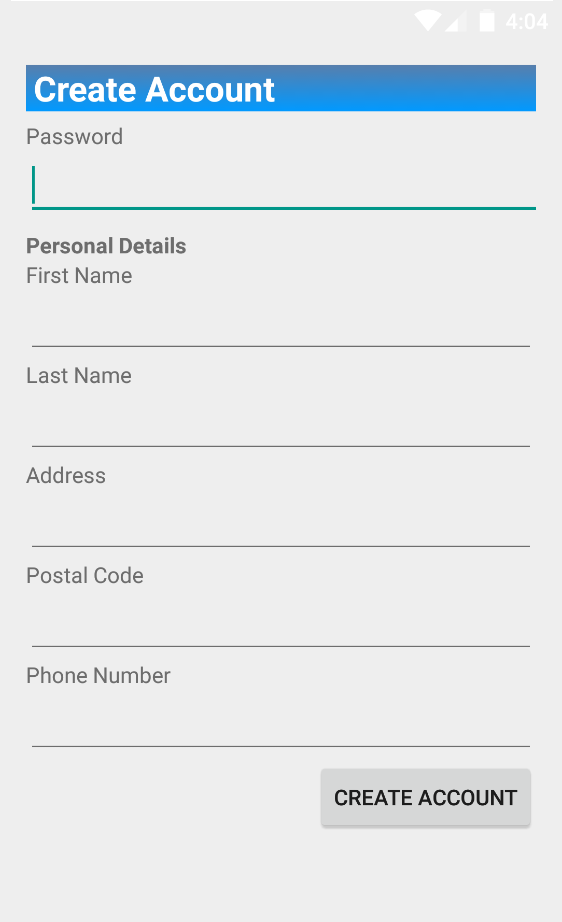
\includegraphics[width=0.5\textwidth]{accountCreation.PNG} 
	\ds{Your filename is accountCreation.PNG not .png, I've fixed it for now.}
\linebreak Figure 2 
\end{center}

The instructions to create an account are as follows: 
\begin{enumerate}
	\item Choose a password between 2-5 characters long.
	\item Enter your first name into the corresponding field.
	\item Enter your last name into the corresponding field.
	\item Enter the first line of your home address as it appears on your mail. Ex: \texttt{125 Royal Ave}
	\item Enter your postal code in the following format: \texttt{L4H 3Y4}
	\item Enter your phone number in the following format: \texttt{4165551911}
	\item Press the \texttt{Create Account} button.
\end{enumerate}

Your Smart-Waiter account has now been successfully created.
\subsection{Accessing Account Settings}
This feature is set to be implemented in our final revision. For the time being, a general walk-through is given using a generic android application settings module. To access your Account Settings in Smart-Waiter proceed with the following steps:

\begin{enumerate}
	\item Press the button with 3 horizontal white lines on the top right-hand corner of the screen to bring up the Navigation menu, as seen 			in Figure 2: 
	\ds{All your figure numbers are wrong}
	\begin{center}
	
\includegraphics[width=0.05\textwidth]{ui-fragment-button.png}
	\linebreak Figure 3
	\end{center}

	\item Press the \texttt{Settings} button in the Navigation Menu as seen 	in Figure 3:

	\begin{center}
	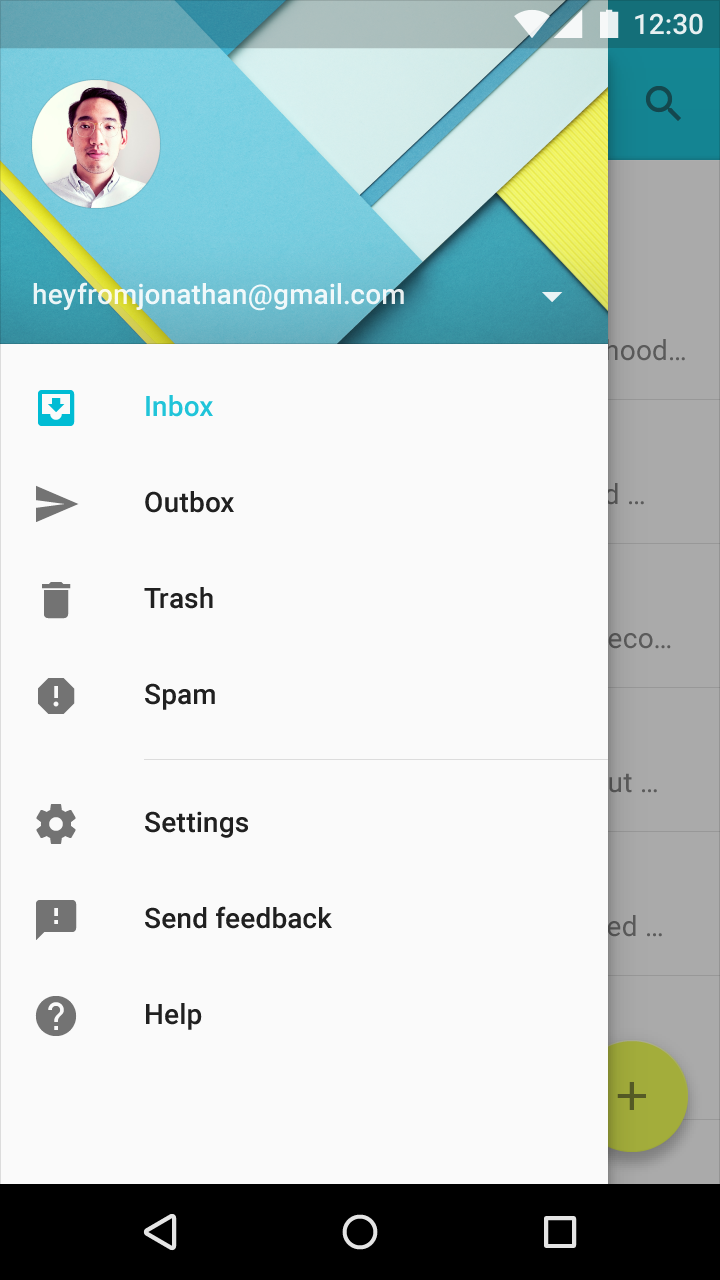
\includegraphics[width=0.4\textwidth]{nav-menu.png}
	\linebreak Figure 4
	\end{center}

\end{enumerate}

From here you can edit your Account Settings. You can perform the following actions in the settings page: \texttt{Change Password} and \texttt{Edit Personal Details}.

\textbf{Changing Your Password:}
	\begin{enumerate}
		\item Press the \texttt{Change Password} label.
		\item Enter your current password into the corresponding field
		\item Press the \texttt{Confirm} button
		\item Enter a new password between 2-5 characters
		\item Enter your new password again into the \texttt{Confirm Password} field
		\item Press the \texttt{Update Password} button.
	\end{enumerate}
	
\textbf{Editing Your Personal Details:}
	\begin{enumerate}
		\item Press the \texttt{Edit Personal Details} label.
		\item Enter your updated information into the corresponding field
		\begin{enumerate}
			\item \textbf{NOTE:} If you leave a field blank, the 						information for the corresponding field will not be updated.
		\end{enumerate}
		\item Press the \texttt{Save Changes} button.
	\end{enumerate}

\section{View Restaurant Menu}
The following section provides step by step process of how to access restaurant menu using Smart-Waiter. As well it provides a detail overview of menu layout.
\subsection{Scanning Barcode}
After logging into Smart-Waiter application, a barcode scanning page will be presented.

\begin{center}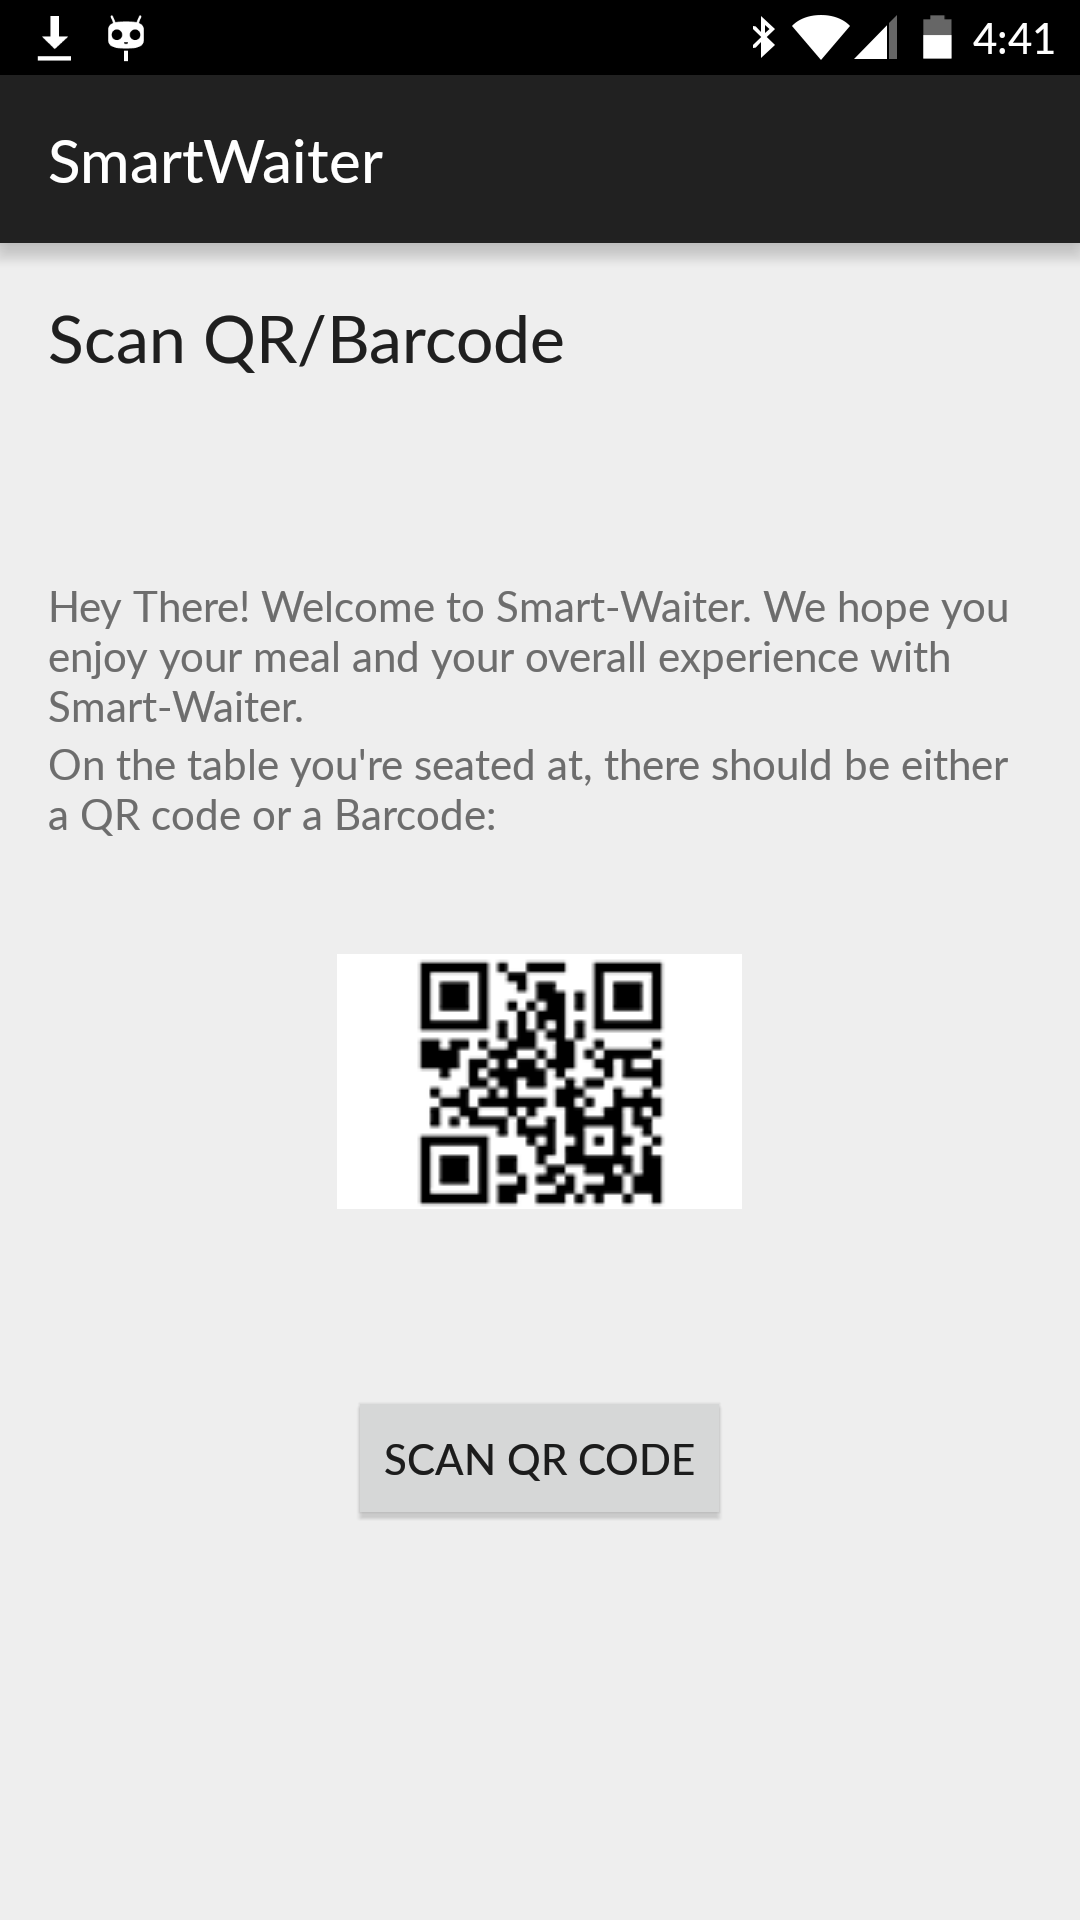
\includegraphics[scale=0.15]{qrcode.png}	\linebreak Figure 5
\end{center}

\noindent To access a restaurant menu, you are required to scan a barcode located within the restaurant. Please follow these instructions to scan the barcode:

\begin{enumerate}
\item In the restaurant, locate the barcode placed on the dining table.
\item Press "Scan QR Code" button on the application. This will open camera page on the user phone. 
\item Proceed to scan the barcode by aligning the red line on screen with the barcode like shown in figure 5.
\begin{center}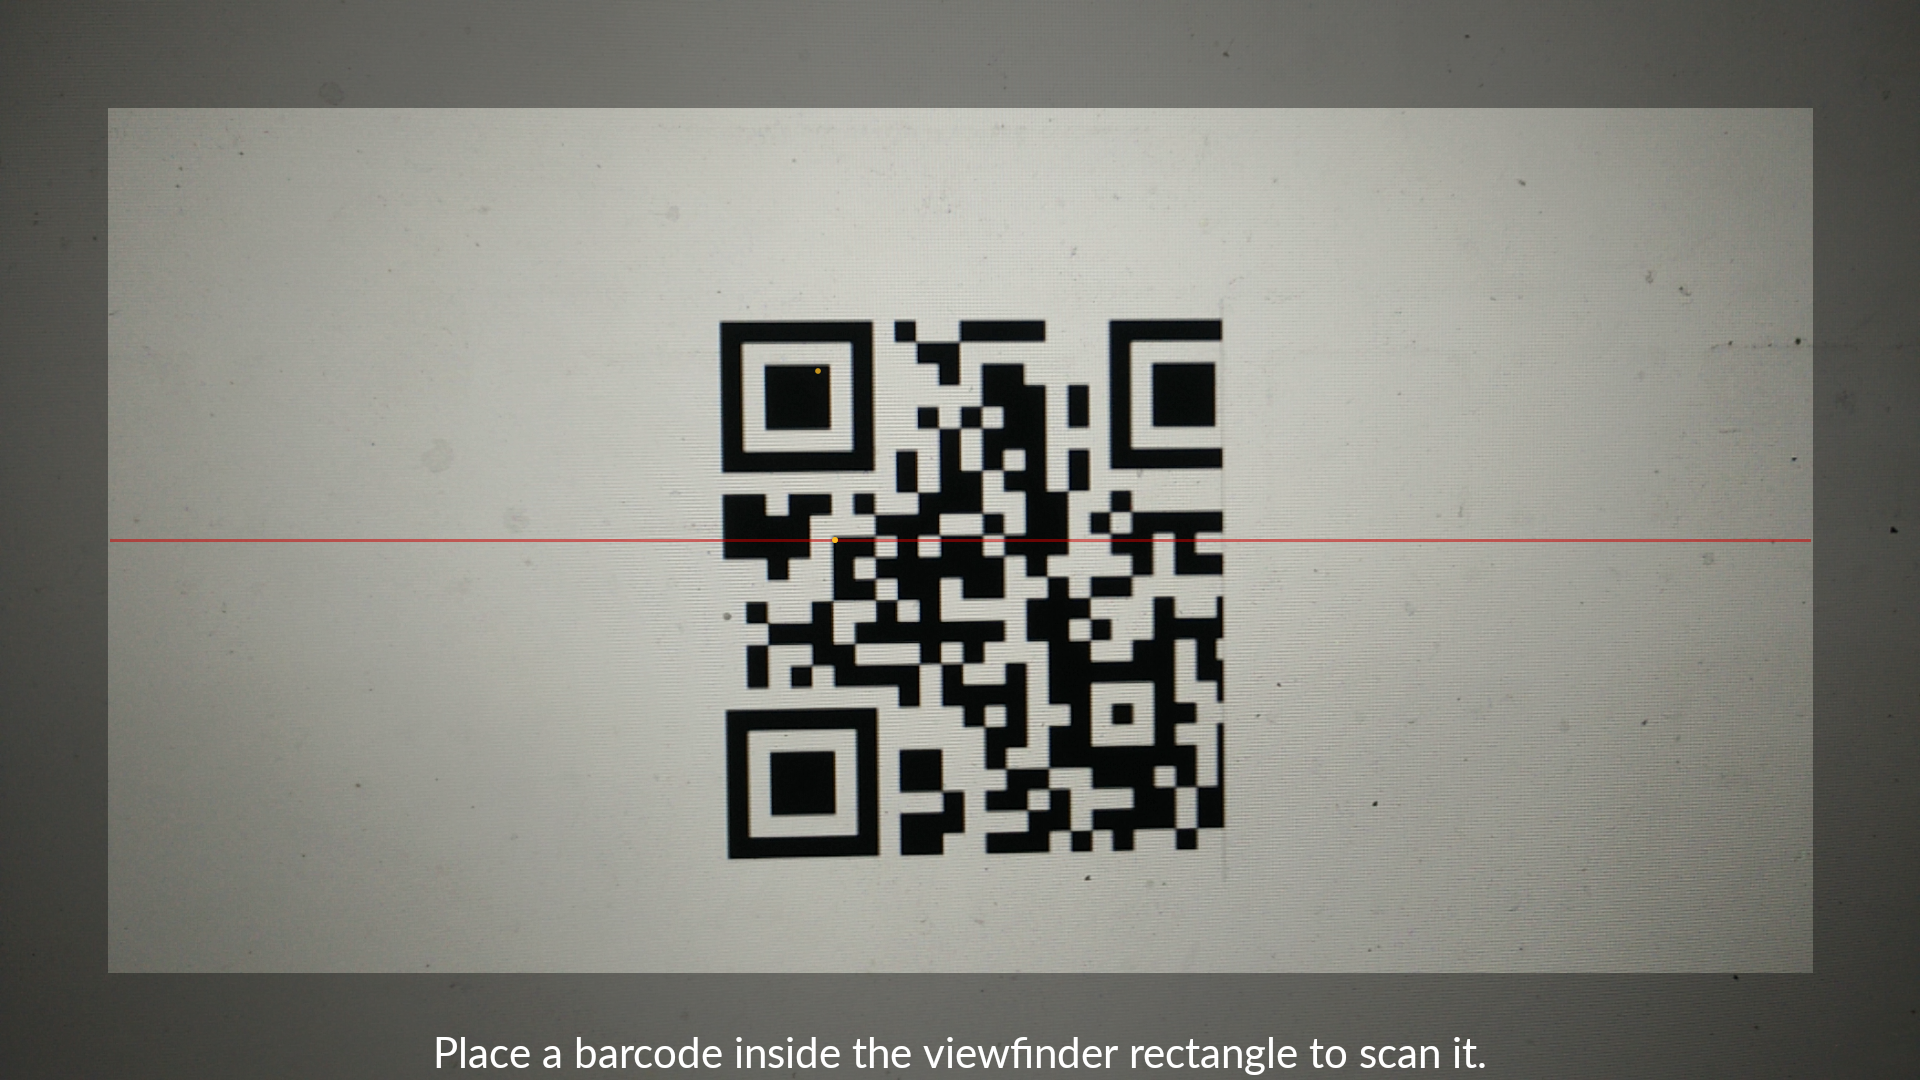
\includegraphics[scale=0.15]{scan.png}	\linebreak Figure 6 \end{center}
\item Wait for the application to recognize the code. 
\end{enumerate}

\noindent If the scan is successful, the application will transition to the menu. Otherwise, the application will transition back to the scan page, and prompt to try again. 
\newline\newline
Please view Section \emph{5.2 - Bug Reporting} if you are having consistent errors scanning the barcode. 

\subsection{Menu Layout}
After successfully scanning a barcode, the application will transition to the restaurant menu. The layout is split into sections as you would see in a typical menu. The following sections are provided and described below.

\subsubsection{Menu Categories}
The first section called upon is menu categories. This is a single page that displays category names of a restaurant menu. Each category contains a list of items available to order at the restaurant.

\begin{center}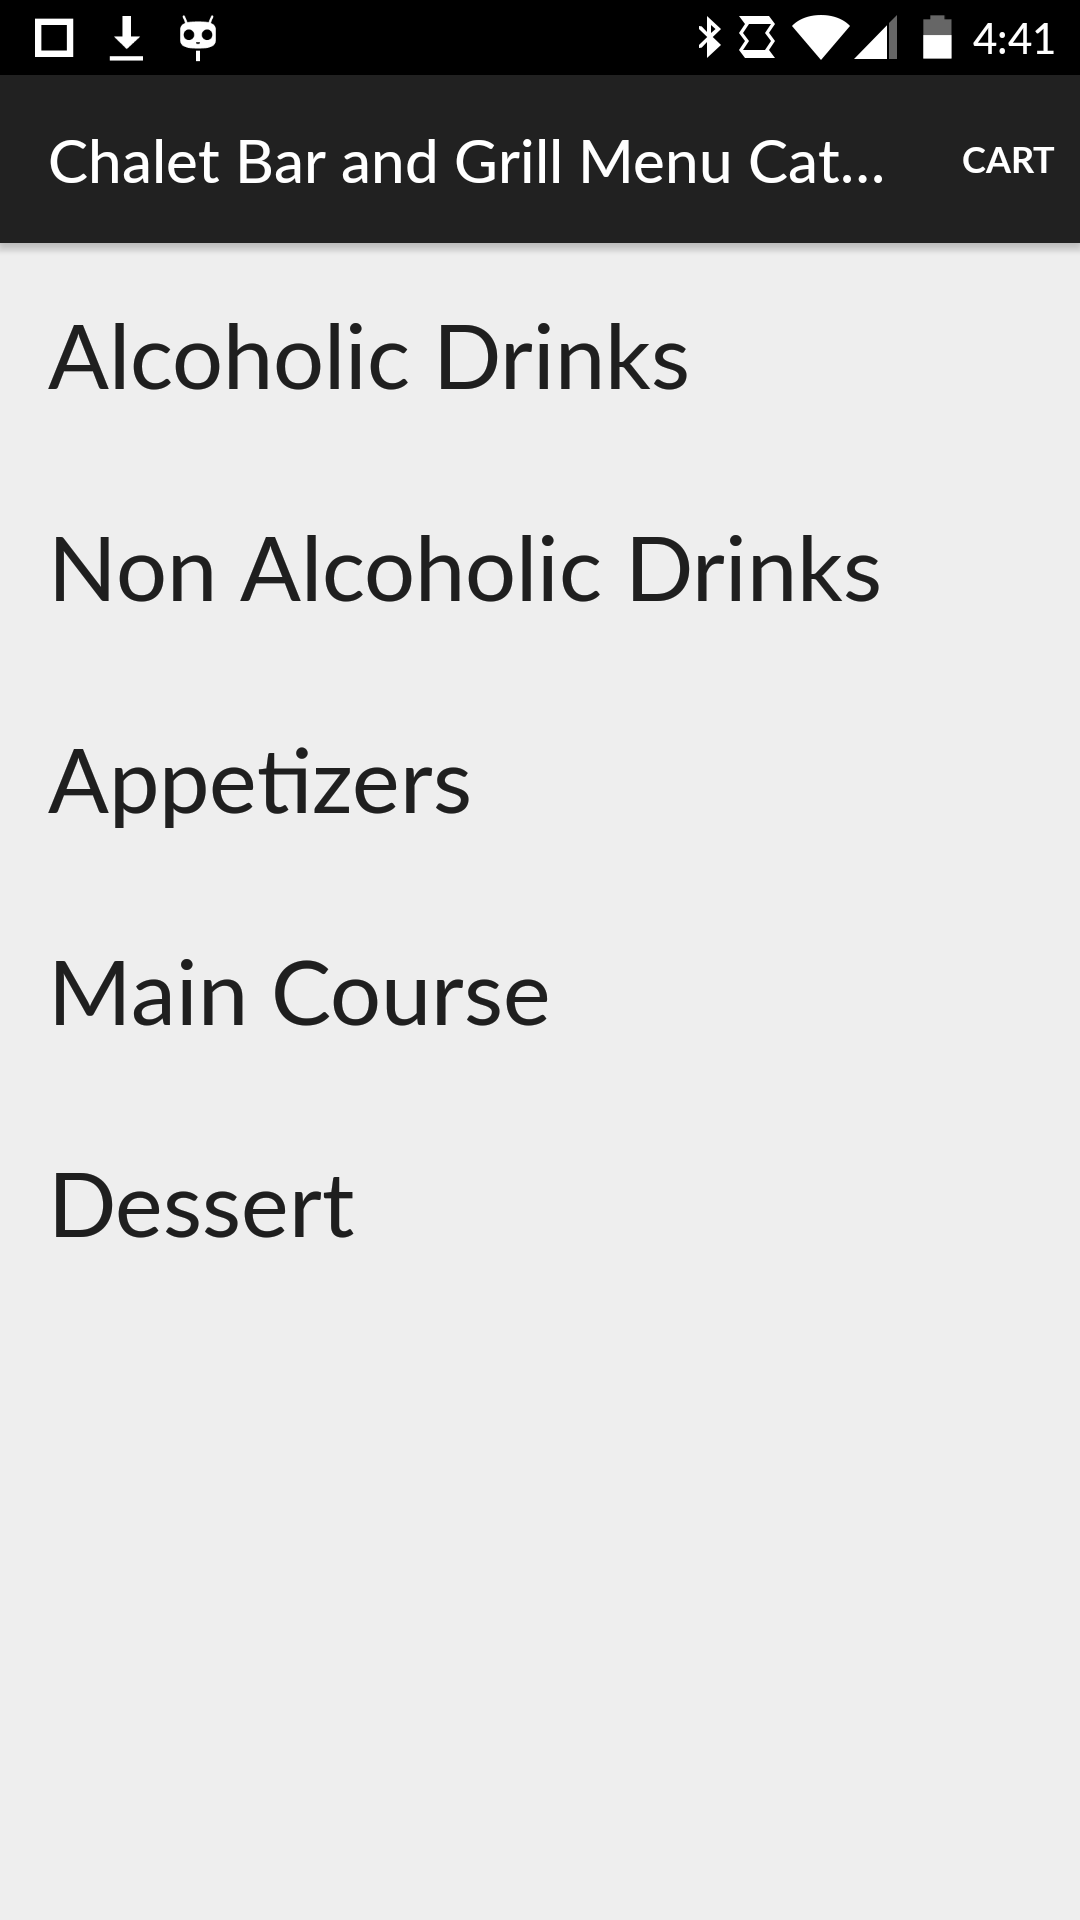
\includegraphics[scale=0.15]{category.png}	\linebreak Figure 7\end{center}

\noindent To view items of a category, tap on the name. This will transition the page to menu items section.

\subsubsection{Menu Items}
This section contains a single page that displays menu items specific to the category selected. To select an item, tap on the row. This will transition to the next section to allow customization of the selected item. 

\begin{center}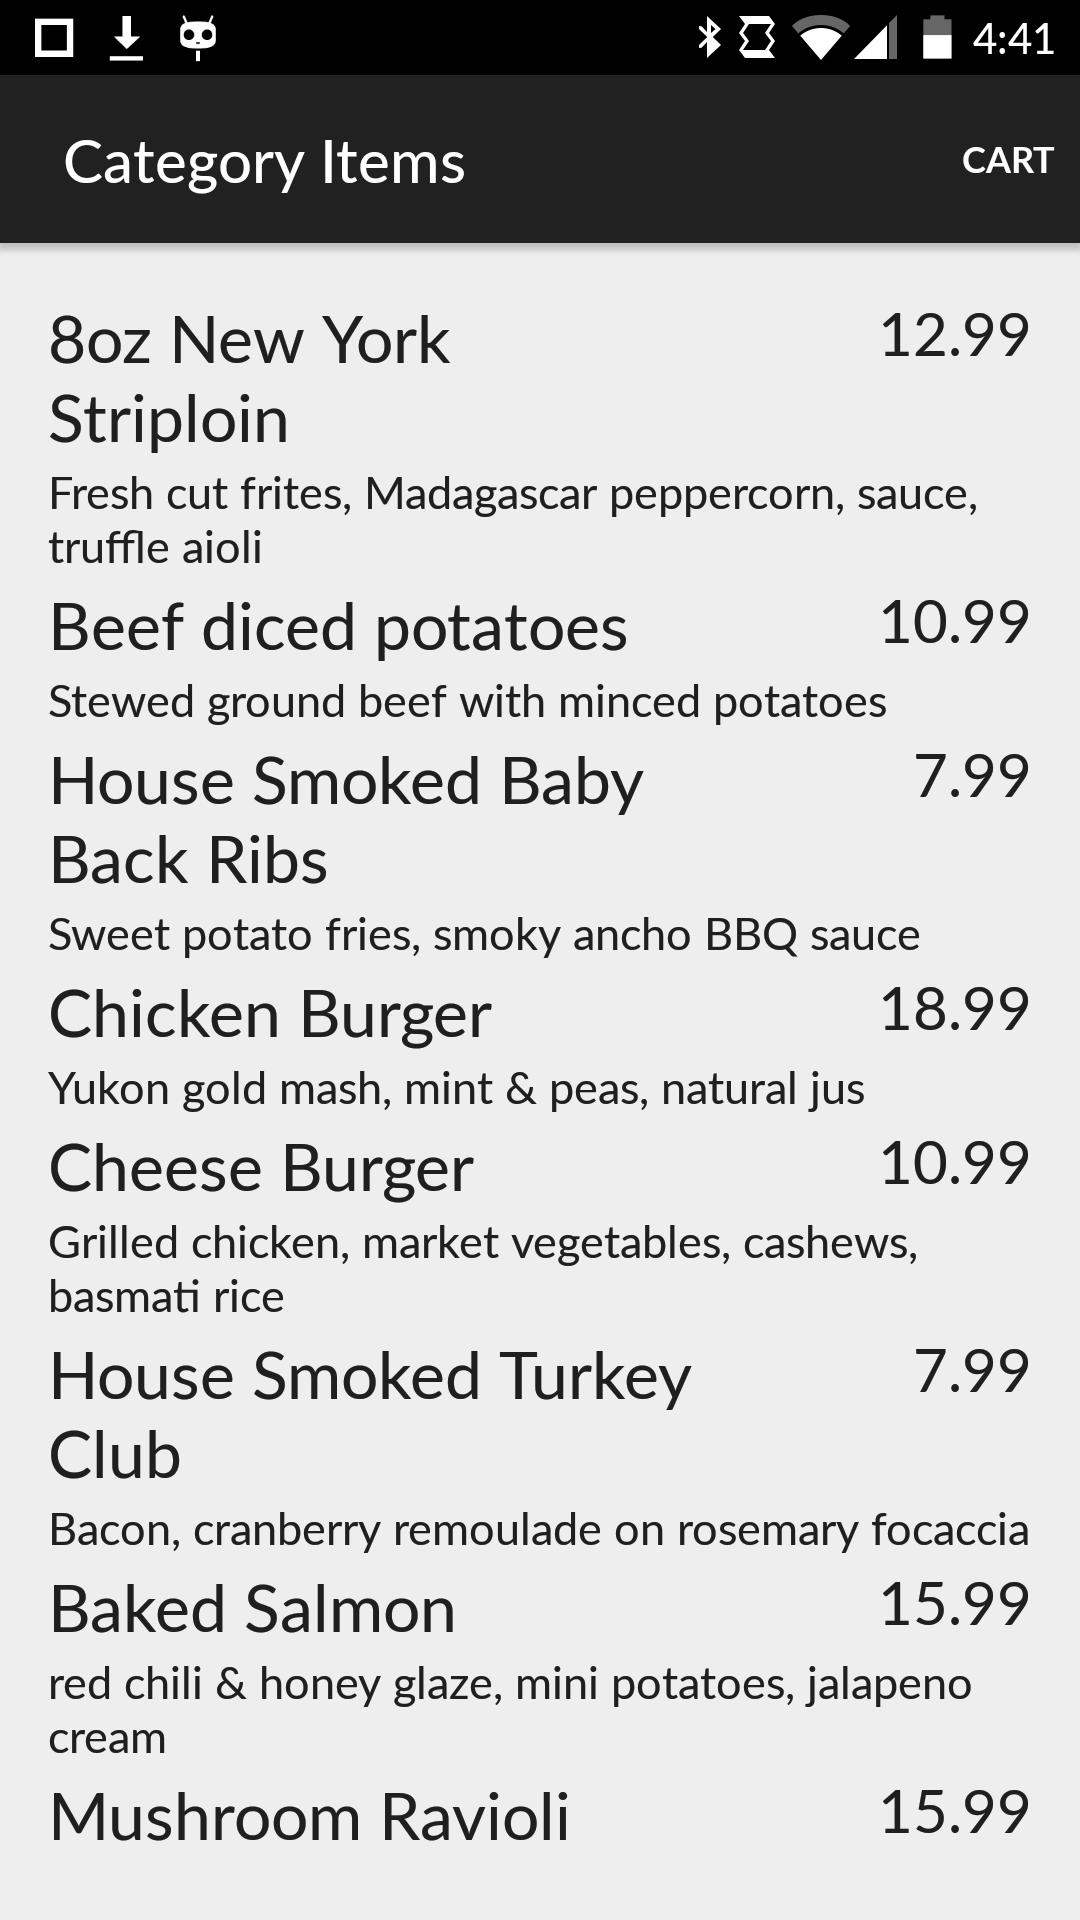
\includegraphics[scale=0.15]{items.png}\end{center}

 
\subsubsection{Customize Item}
There are three different methods available to customize an item. 

\begin{enumerate}
  \item Custom Toppings
  \item Custom Sides
  \item Special Instructions
\end{enumerate}

\noindent  Each method is presented on a separate page, and is shown in accordance to the item selected. This means, that you will have the ability to customize the item by choosing toppings, picking a side and by setting special instructions if applicable. 
\newline \newline
The layout of the page, and use of each method is provided below: \pagebreak\newline
\textbf{Custom Toppings} \newline
If toppings are available to add to the item, the following page is presented:
\begin{center}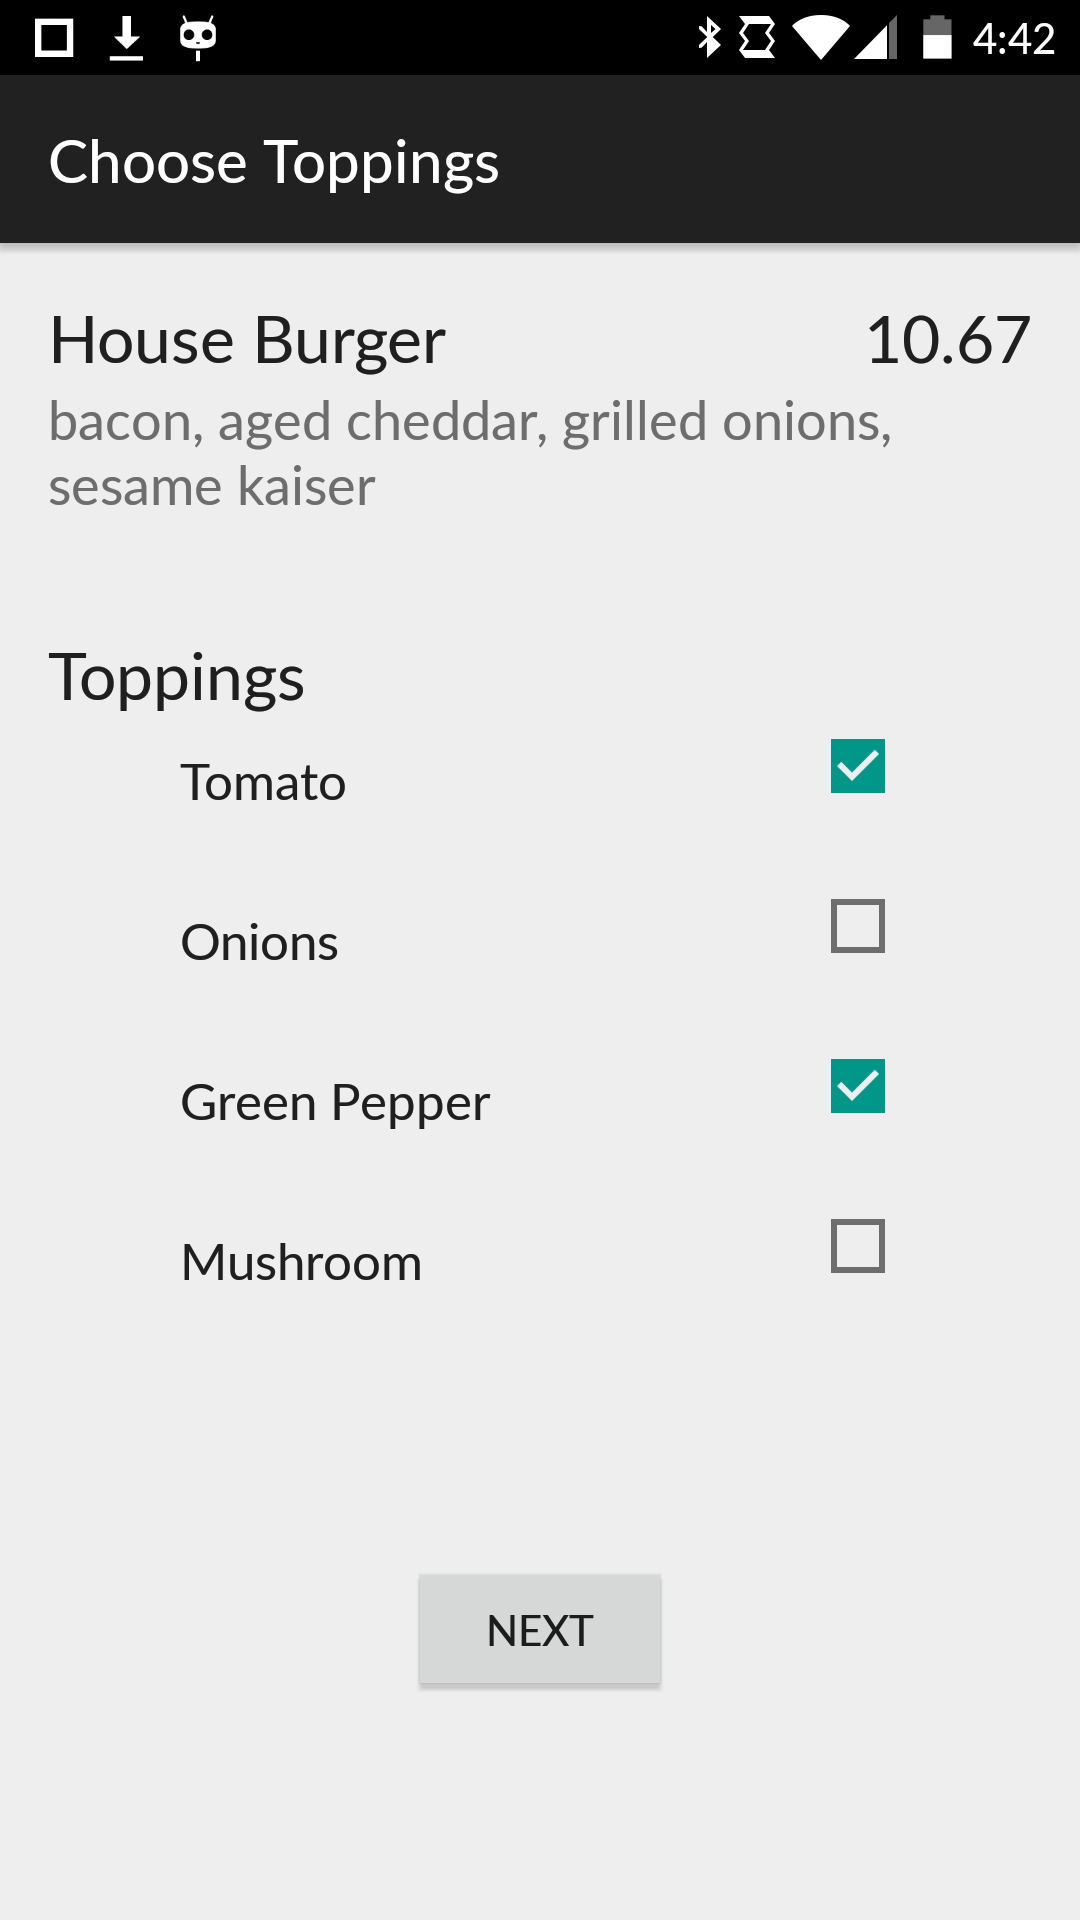
\includegraphics[scale=0.15]{toppings.png}	\linebreak Figure 8 \end{center}
This page displays a list of toppings available. To add a topping, tap on the check box to the right of the topping name. Multiple toppings can be selected. When complete, press "Next" button on the bottom of the page to proceed.\pagebreak
\newline
\textbf{Custom Sides}\newline
If the item selected is offered a side, the following page is displayed:
\begin{center}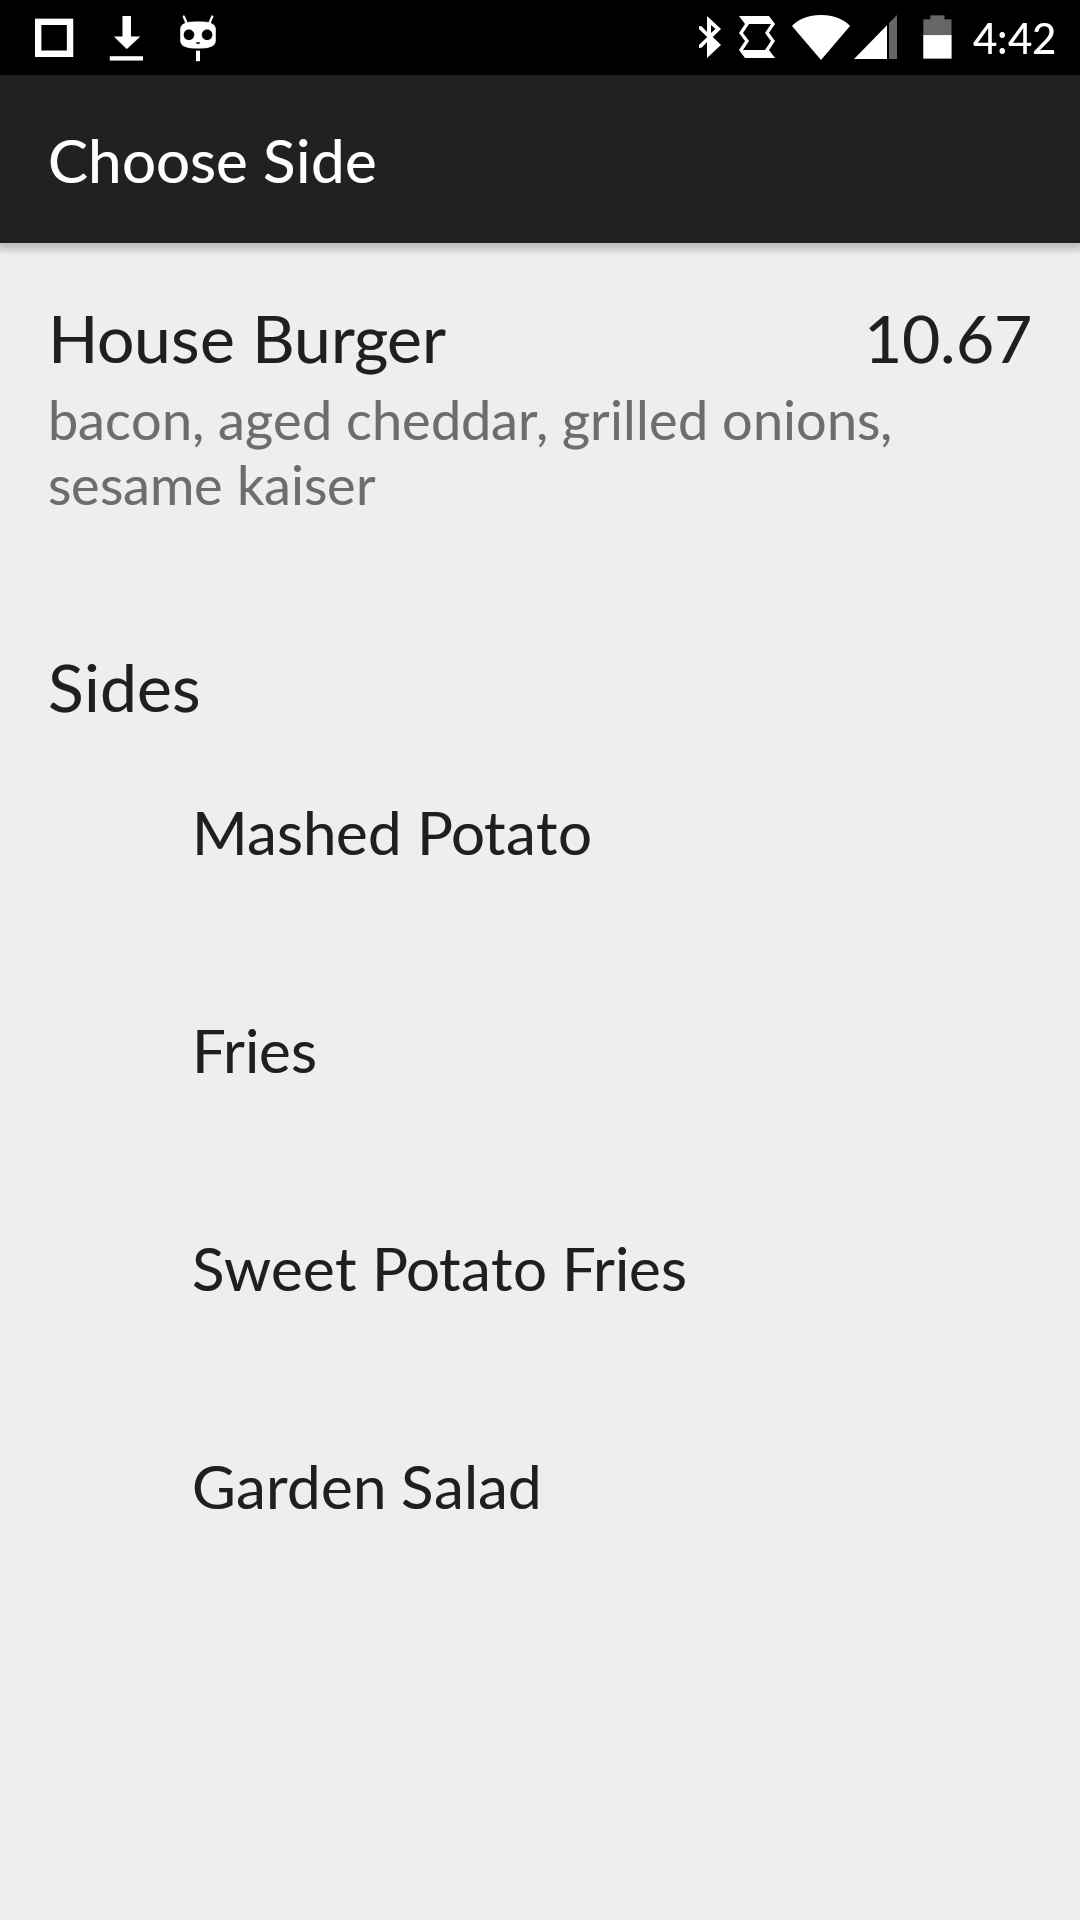
\includegraphics[scale=0.15]{sides.png}	\linebreak Figure 9\end{center}
This page is used to select a side dish for an item. Side dish names are presented in a list. To select a side dish, simply tap on its name.\pagebreak \newline
\textbf{Special Instructions}\newline
For all menu items, special instructions can be requested. To make a request, tap on the text field under "Special Instructions", and enter your text. 
\begin{center}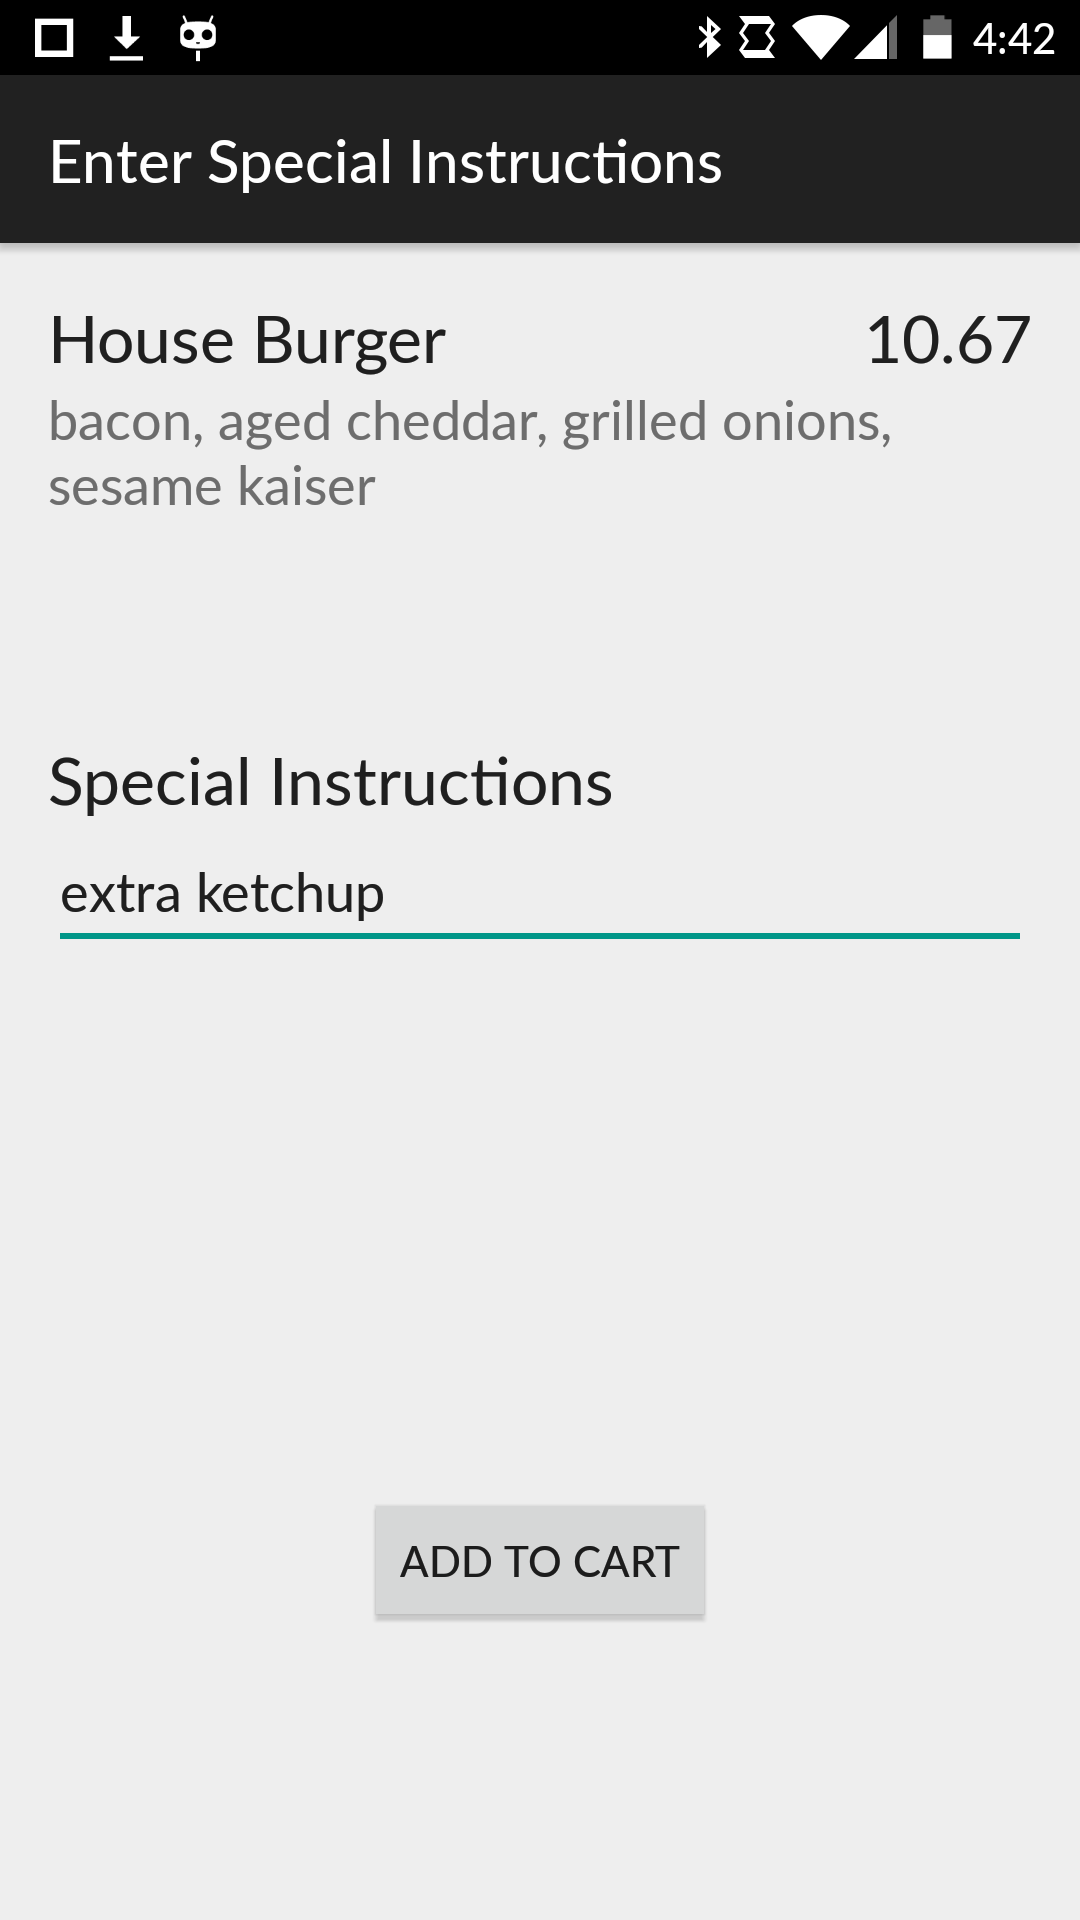
\includegraphics[scale=0.15]{instructions.png}	\linebreak Figure 10\end{center}
Once complete, tap "Add to Cart" button on the bottom of the page. This will add the selected item to cart, and transition the page back to menu items section. 

\subsubsection{Menu Cart}

Menu cart section contains all items selected to order. During any section after scanning the barcode, you can view your cart by tapping "Cart" on the title bar.
\begin{center}
\includegraphics[scale=0.15]{titlebar.png}	\linebreak Figure 11\end{center}

\noindent Doing so will transition the page to cart page. Every item selected is presented in sequent rows on this page. Specifically, the item name, price, and custom details are provided for review. There are several options available on this page:

\begin{itemize}
  \item C - Customize item: Pressing this button allows  you to modify the item
  \item D - Delete item: Pressing this button will remove item from cart
  \item Confirm Order: Pressing this button will transition to payment page
\end{itemize}

\begin{center}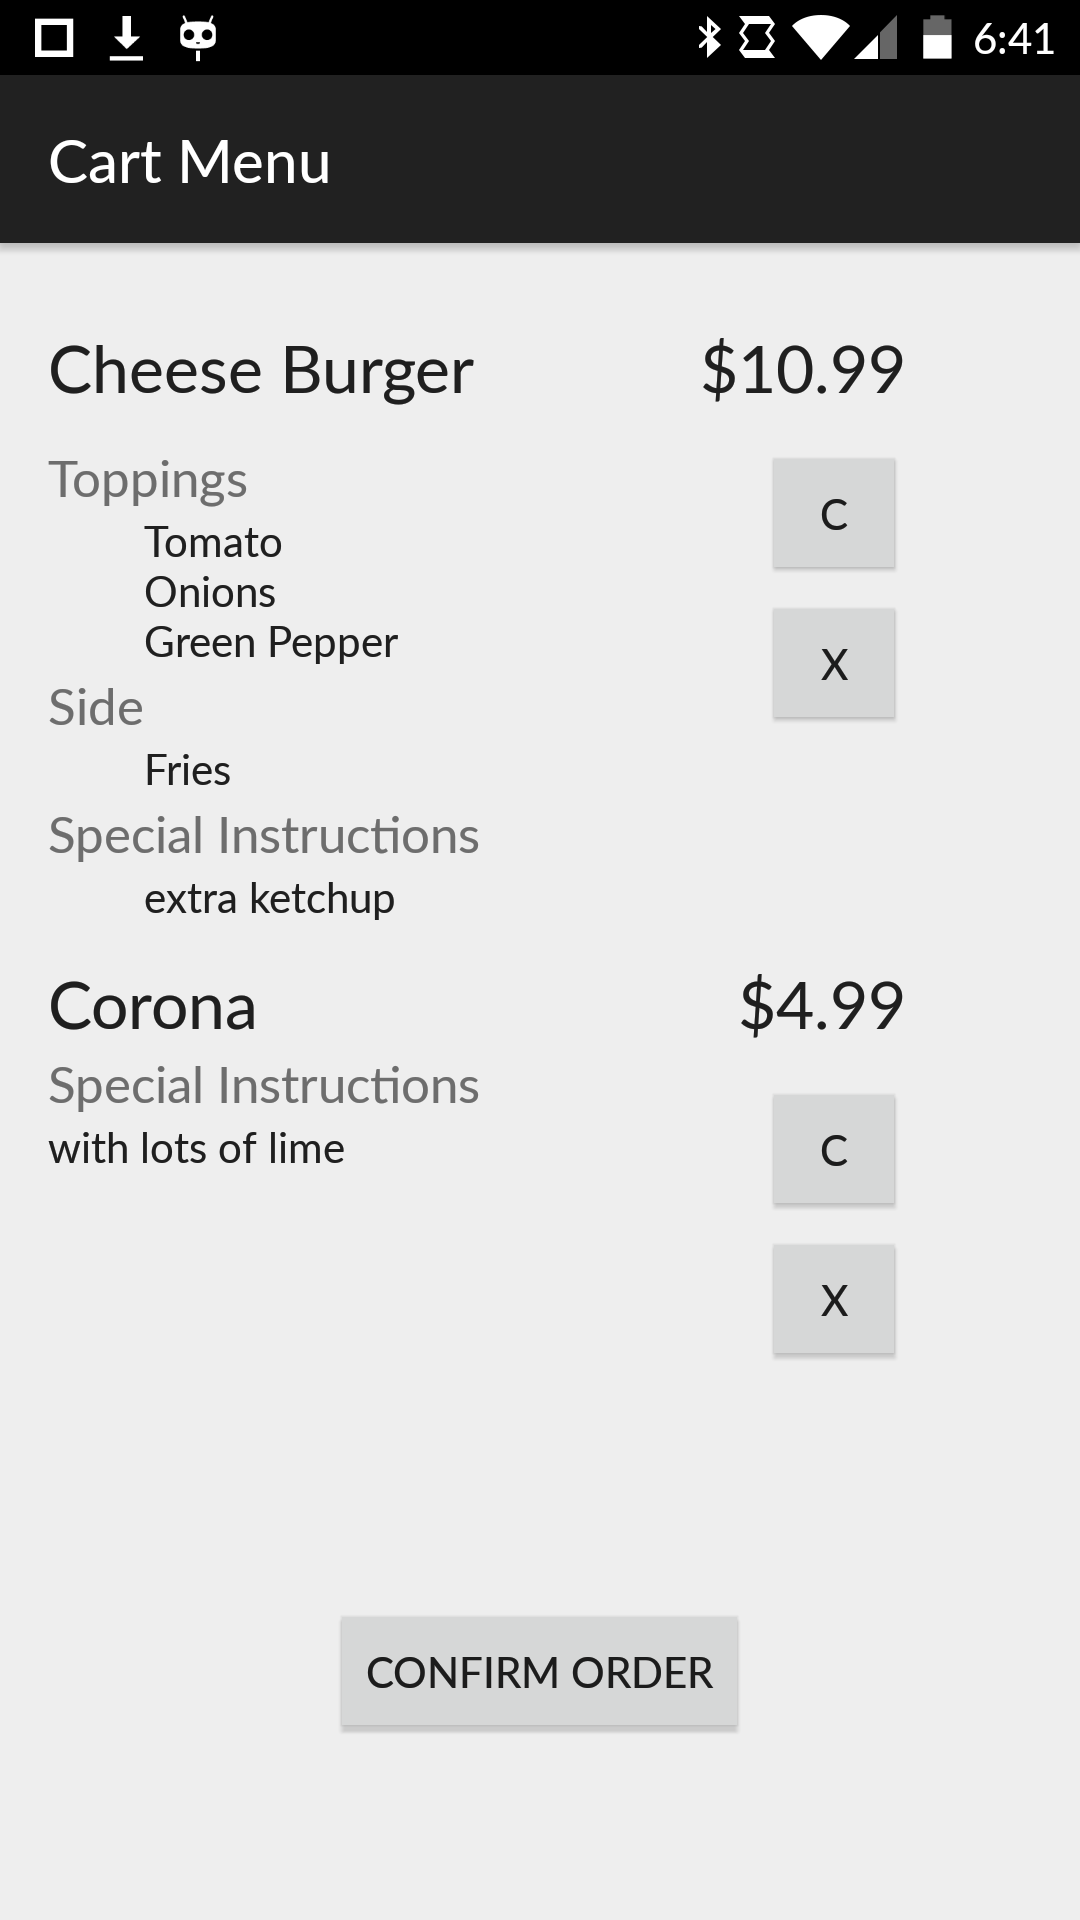
\includegraphics[scale=0.15]{cart.png}	\linebreak Figure 12\end{center}

\section{Placing an Order}
The following section provides a step by step example of placing an order. If you have not already, it is advised you review \emph{View Restaurant Menu} section before proceeding to avoid confusion. 
\subsection{Adding Item to Cart}
This section will walk-through how to add an item to your cart. In this case we are using the Chalet Bar and Grill Menu, however these instructions can be applied to any menu available through Smart-Waiter. Your screen will look similar to Figure 4 below. To learn how to add an item to your cart, proceed with the following instructions:
	\begin{enumerate}
		\item Press the label for the category of your choice. Ex: 						\texttt{Appetizers}

	\begin{center}
		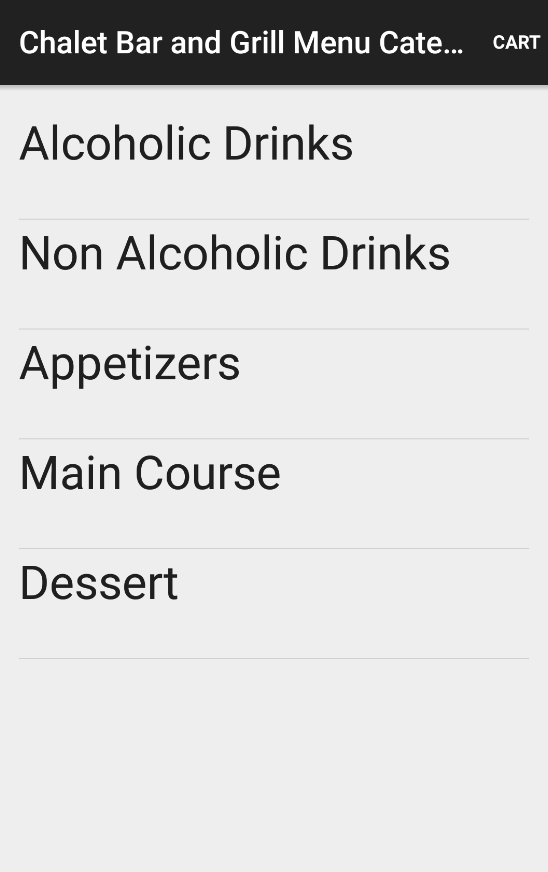
\includegraphics[width=0.5\textwidth]{main-menu.png}
		\linebreak Figure 13
	\end{center}

		\item Press the label for the menu item of your choice. Ex: 					\texttt{Autumn Spinach Salad}
		\begin{center}
			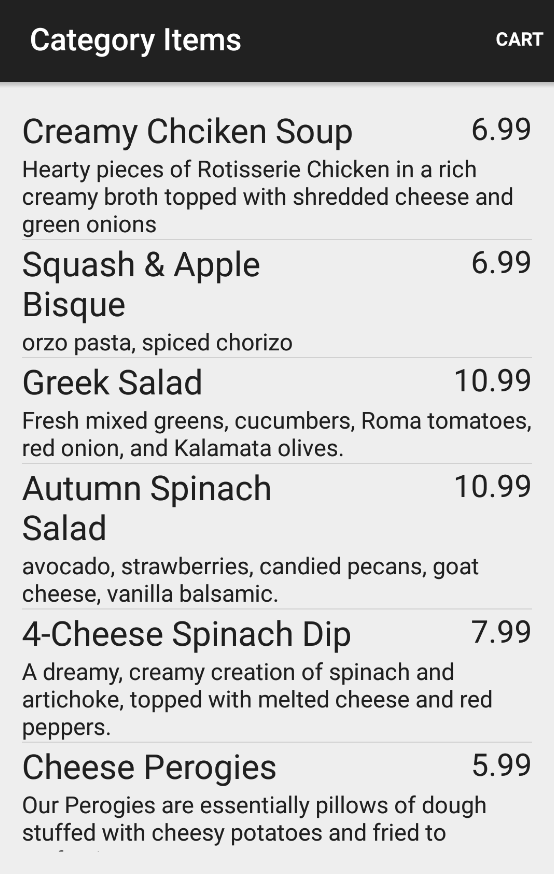
\includegraphics[width=0.5\textwidth]{appetizers.png}
			\linebreak Figure 14
		\end{center}				
		
		\item Given the selected item, the only means of customization is special instructions. Thus, enter any special instructions you may have for the menu 					item. Ex: \texttt{Easy on the salad dressing} - Refer to Figure 			6
		\begin{center}
			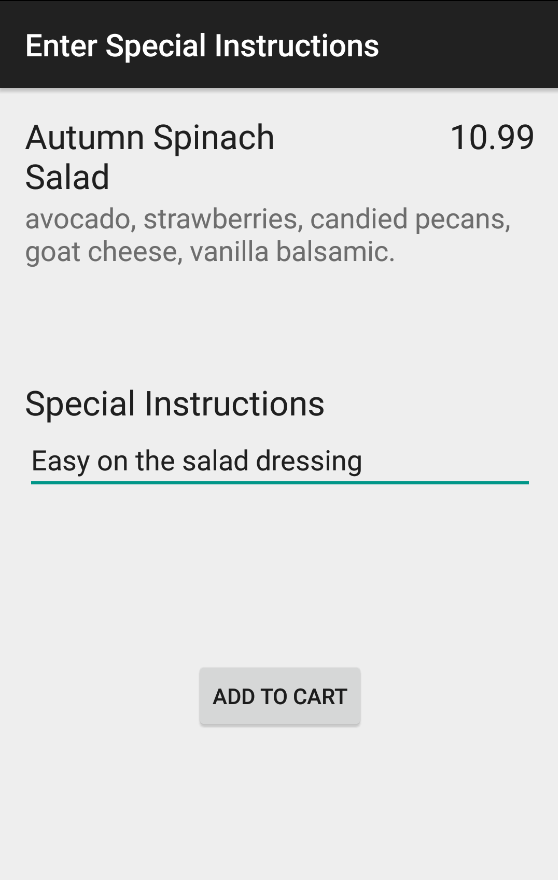
\includegraphics[width=0.5\textwidth]{special-instructions.png}
			\linebreak Figure 15
		\end{center}		
	
		\item Press the \texttt{Add To Cart} button
	\end{enumerate}

\subsection{Order Confirmation}
This section will guide you through the order confirmation process. We will continue with the Chalet Bar and Grill case we followed in the previous sections. These instructions can be applied to any menu available through Smart-Waiter. To learn how to confirm your order, proceed with the following instructions:

	\begin{enumerate}
		\item Press the \texttt{Cart} button on the top right corner of the 			application.
		\item Press the \texttt{Confirm Order} button
		\begin{center}
			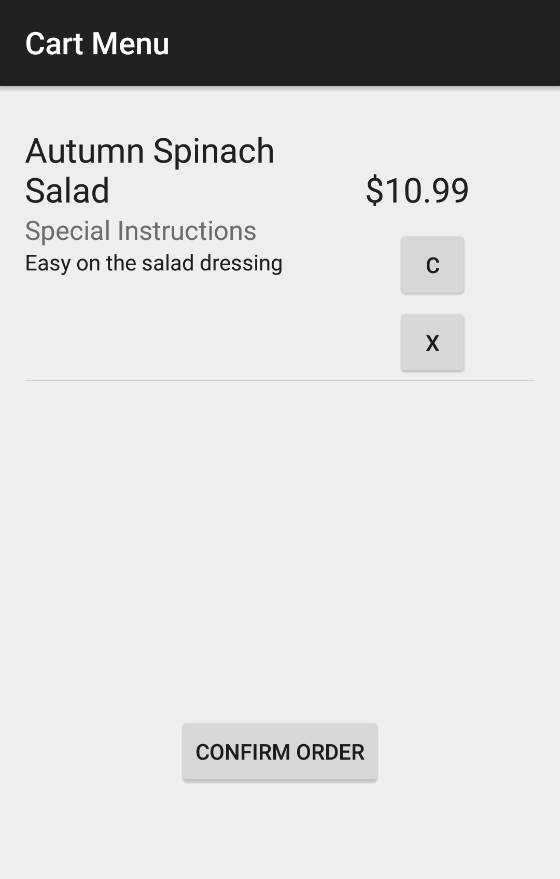
\includegraphics[width=0.5\textwidth]{confirm-order.png}
			\linebreak Figure 16
		\end{center}
		\item Press the \texttt{Proceed to Payment} button
	\end{enumerate}
	
	\textbf{Edit Special Instructions:}
	To edit the special instructions for a menu item, proceed to the Cart Menu by pressing the \texttt{Cart} button on the top right corner of the screen and follow these instructions:
	
	\begin{enumerate}
		\item Press the \texttt{C} button
		\item Update the \texttt{Special Instructions} field with your new instructions
		\item Press the \texttt{Modify Item} button
	\end{enumerate}
	
		\textbf{Remove Item from Cart:}
	To remove a menu item from your cart, proceed to the Cart Menu by pressing the \texttt{Cart} button on the top right corner of the screen and follow these instructions:
	
	\begin{enumerate}
		\item Press the \texttt{X} button
	\end{enumerate}

\subsection{Paying for an Order}
This section will guide you through the payment process. If you have not read the \emph{Order Confirmation} section yet, please do so now before moving forward with this guide. This tutorial assumes that you have added at least one menu item to your cart and have followed the main \emph{Order Confirmation} instructions up to step 3 where the user presses the \texttt{Proceed to Payment} button step. Your screen will look similar to Figure 8 below. To learn how to pay your order, proceed with the following instructions:

	\begin{center}
		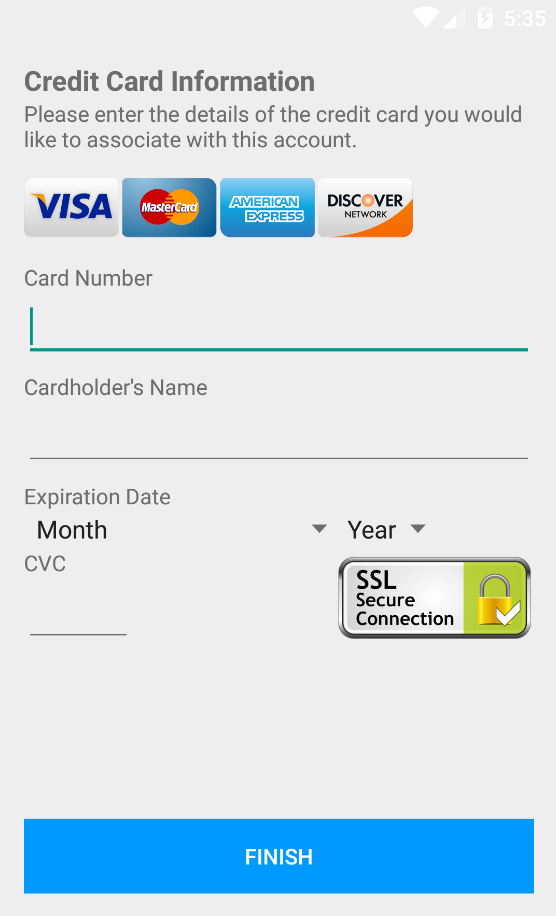
\includegraphics[width=0.5\textwidth]{cc.png}
		\linebreak Figure 17
	\end{center}
	\begin{enumerate}
		\item Enter your \emph{Credit Card Number} into the \texttt{Card 				Number}	field
		\item Enter the \emph{Cardholder's Name} into the corresponding 				field
		\item Enter the \emph{Expiration Date} using the dropdown list
		\item Enter the \emph{CVC} into the corresponding field
		\item Press the \texttt{Finish} button
	\end{enumerate}

\subsection{Submitting an Order}
Once Finished is pressed as per Section 4.3, the order is placed immediately. A confirmation message will appear at the bottom of the page to alert the user.  \emph{Please note that this order is final and can no longer be modified.}

\section{Troubleshooting}
\subsection{Generic Troubleshooting}
In the rare event in which the application does not respond please follow the following steps;
\begin{enumerate}
	\item Try to restart the application
	\item If restarting the application does not work, then please restart your android device.
	\end{enumerate}
	If none of these steps work, please use the bug-reporting feature if available. If this feature is not available, send an email directly to our system admin customer-service@smartwaiter.ca.\\\\
	Note:  \emph{Most errors will provide meaningful feedback and guide the user to resolve the issue. In these cases its best to follow the steps mentioned in the error.}
\subsection{Bug Reporting}
The bug-reporting feature has been implemented for the users convenience. There is an icon for bug reporting, located on the barcode-scanning screen (to be implemented for final version). This icon looks as follows;\\
\begin{center}
	
\includegraphics[width=0.5\textwidth]{bugReport.png}
	\linebreak Figure 18
\end{center}
Users can report bugs or any other issues by utilizing this button. Simply click on this button, and you will be prompted for information regarding the bug. Once you have provided as much information as possible, click send and our customer support will get back to you within 4 hours.\\\\
Note:  \emph{Please follow section 5.1 before reporting any bugs.  In majority of the cases, the steps listed in this section can successfully resolve most issues.}
\subsection{Frequently Asked Questions}
\begin{enumerate}
	\item \emph{Can I use Smart-Waiter when there is no network connectivity?}\\\\
	You can still use the application to view menus. However, in order to submit your order and pay, you will be required to have network connectivity.
	\item \emph{Can I use Smart-Waiter application on any other platform?}\\\\
	No, currently this application is only available for Android.
	\item \emph{What if I want to move tables after placing an order?}\\\\
	You need to notify the restaurant if you move tables, so that your food can be delivered to your new table.
	\item \emph{My orders are not going through, whom should I contact?}\\\\
	Contact our customer support directly at customer-service@smartwaiter.ca or use "bug reporting" feature as per section 5.2. Please do not ask the restaurants to troubleshoot issues.
	\item \emph{I do not have a credit card; can I still use the application?}\\\\
	No the application requires a credit card to pay for your meals. There is no other option to pay.
	\item \emph{Can I split the bill with my friend?}\\\\
	No, this application does not support splitting the bill. However, you and your friend can both be seated at the same table, and use the application to order from two different devices. 
	\item \emph{What if, I do not want to provide personal information for this application?}\\\\
	Personal information is only used to send out promotion codes and perform data analytics for the restaurant. If you are not comfortable, you can simply leave these fields blank when 	   creating an account.
	\item \emph{How do I change my account information?}\\\\
	You can always change your account information through the settings gear icon on the barcode-scanning screen.
	\item \emph{Can I place multiple orders from same table?}\\\\
	Yes, you can place multiple orders from multiple devices from the same table. There are no extra fees associated with this. 
	\item \emph{Why can't \ds{I? We? Someone?}
	see some of the deals in the restaurant through the application?}\\\\
	This can occur if the restaurant has not uploaded their latest data to the application. Please be sure to report this bug and we will follow up on it.
\end{enumerate}
	

\ds{Why are some figures colour and others grayscale?}


\end{document}